\chapter{Basic Components in a Distributed Storage Service}
A distributed storage system is designed to store and manage vast amounts of data reliably and efficiently. The system is composed of several key components that work together to ensure scalability, fault tolerance, and high performance. In this chapter, we break down the major components, provide further details on their roles, and illustrate each with real-world examples.

\begin{figure}[htbp]
  \centering
  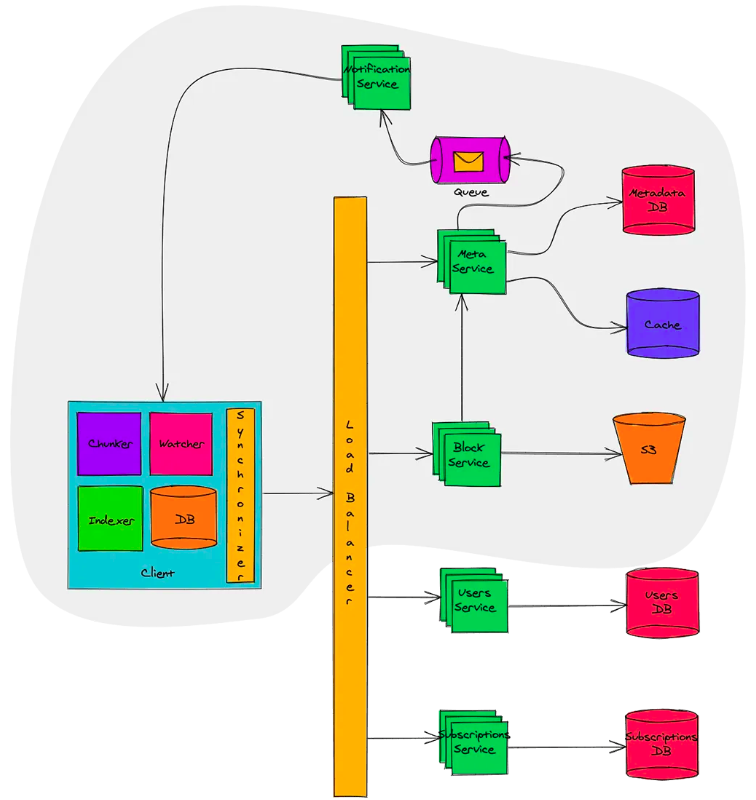
\includegraphics[width=0.8\textwidth]{img/architecture.png}
  \caption{A distributed storage architecture, illustrating the interaction between various components. The client interacts with the load balancer when making requests. The load balancer distributes different requests to the metadata service, block service, and database. The metadata service manages the metadata and interacts with the notification service to send updates. The block service handles the actual data storage and retrieval, while the database stores structured data related to the system's operation and user credentials. The notification service provides real-time updates to clients and other components. [Source: \cite{Dropbox_solution2}]}\label{fig:architecture}
\end{figure}


\section{Client}
The \textbf{Client} is the primary interface through which users interact with the storage system. It can be implemented in multiple forms:
\begin{itemize}
    \item \textbf{APIs and Protocols:} Clients may use HTTP, gRPC, or other APIs to communicate with the storage backend. For example, a developer might use RESTful APIs to integrate the storage service into their application.
    \item \textbf{Web Interface:} End users can interact with the system via a browser-based interface, providing ease of access and management.
    \item \textbf{Daemon Processes:} Applications like Dropbox use background daemon processes to monitor file system changes. This process automatically synchronizes files across devices by detecting updates and uploading or downloading files as needed.
\end{itemize}
\textbf{Example:} When a user modifies a file on their computer, the client-side daemon detects this change and triggers an upload request via the API, ensuring that the most current version is stored and replicated across devices.

\section{Frontend Server}
The \textbf{Frontend Server} acts as the gateway to the distributed storage system. Its responsibilities include:
\begin{itemize}
    \item \textbf{Handling Client Requests:} It receives and processes incoming requests, authenticating and authorizing users.
    \item \textbf{Session Management:} It maintains session states to ensure that client interactions remain consistent and secure.
    \item \textbf{Request Routing:} It forwards requests to the appropriate backend components, such as storage or metadata services.
\end{itemize}
\textbf{Example:} In a cloud storage platform, the frontend server might receive an HTTP request to upload a file. It then validates the user session, checks permissions, and routes the request to the backend servers responsible for handling the file storage.

\section{Metadata Service}
The \textbf{Metadata Service} is critical for managing the information about the stored data:
\begin{itemize}
    \item \textbf{Metadata Storage:} It holds metadata such as file size, creation date, permissions, and file block information.
    \item \textbf{Access Control:} Metadata is used to enforce security policies and access rights.
    \item \textbf{System Scalability:} By efficiently managing metadata, the system can quickly locate and retrieve data blocks, which is essential for large-scale storage environments.
\end{itemize}
\textbf{Example:} In the Hadoop Distributed File System (HDFS), the NameNode functions as the metadata service, tracking where each block of data is stored across the cluster.

\section{Notification Service}
The \textbf{Notification Service} provides real-time communication between components:
\begin{itemize}
    \item \textbf{Asynchronous Messaging:} It sends alerts, status updates, or error notifications to various services.
    \item \textbf{Client Updates:} It can notify clients about changes, such as the status of file block uploads or replication progress.
\end{itemize}
\textbf{Example:} When a large file is being split and distributed across several storage nodes, the notification service can update the client on the progress, ensuring transparency and timely error handling if issues arise.

\section{Block Service}
The \textbf{Block Service} is responsible for the physical storage and management of data blocks:
\begin{itemize}
    \item \textbf{Data Chunking:} Large files are split into manageable blocks, which are stored separately to improve retrieval efficiency and fault tolerance.
    \item \textbf{Redundancy and Replication:} To ensure high availability, blocks are often replicated across multiple nodes.
\end{itemize}
\textbf{Example:} In systems like Amazon S3 or HDFS, the block service handles the distribution and replication of file chunks, ensuring that data remains accessible even if one node fails.

\section{Database}
The \textbf{Database} component stores structured data related to the system's operation:
\begin{itemize}
    \item \textbf{Structured Data Management:} This includes information such as user credentials, access logs, and configuration settings.
    \item \textbf{Distributed Databases:} To achieve high availability and scalability, databases in distributed systems are often replicated across nodes.
    \item \textbf{Types:} Both SQL (e.g., MySQL, PostgreSQL) and NoSQL (e.g., Cassandra, MongoDB) databases are employed based on the use-case requirements.
\end{itemize}
\textbf{Example:} A metadata repository may use a NoSQL database for rapid query performance and horizontal scaling, while a transactional logging system might rely on a relational SQL database for ACID-compliant operations.

\section{Load Balancer}
The \textbf{Load Balancer} distributes network traffic evenly across multiple servers:
\begin{itemize}
    \item \textbf{Traffic Distribution:} It prevents any single server from becoming a bottleneck by spreading out incoming requests.
    \item \textbf{Fault Tolerance:} In case one server goes down, the load balancer redirects traffic to healthy servers.
    \item \textbf{Algorithms:} Common strategies include round-robin, least connections, and IP hash.
\end{itemize}
\textbf{Example:} A load balancer might be used to distribute client requests across several frontend servers, ensuring that no single server becomes overwhelmed during peak usage times.

\section{Message Queues}
\textbf{Message Queues (MQ)} enable asynchronous communication between distributed system components:
\begin{itemize}
    \item \textbf{Decoupling Services:} They allow different parts of the system to operate independently by queuing messages for later processing.
    \item \textbf{High Throughput:} MQs are designed to handle large volumes of messages efficiently.
    \item \textbf{Common Technologies:} Examples include RabbitMQ, Apache Kafka, and Amazon SQS.
\end{itemize}
\textbf{Example:} In a distributed storage system, a message queue can handle tasks like file processing and replication requests, ensuring that these tasks are processed in an orderly and fault-tolerant manner.

\section{Cache}
A \textbf{Cache} is a high-speed data layer used to store frequently accessed data:
\begin{itemize}
    \item \textbf{Latency Reduction:} Caches help reduce the time required to access data, thereby improving overall system performance.
    \item \textbf{Resource Optimization:} By storing temporary data, caches help reduce the load on backend systems.
    \item \textbf{Technologies:} Common caching solutions include Redis and Memcached.
\end{itemize}
\textbf{Example:} Frequently accessed metadata or small file fragments might be stored in a Redis cache, ensuring that user queries are served rapidly without repeatedly accessing slower backend storage.
